\documentclass[]{article}
\usepackage{graphics}
\usepackage{graphicx}
\usepackage{tabularx}
\usepackage[titletoc,title]{appendix}


\begin{document}


 \section{ Overview of experiments}
 \subsection{Overview of neutron form factor experiments}
 Both neutron form factor experiments measure quasi-free scattering on a nuclear target. The standard Hall~A
 BigBite Spectrometer is used to detect the scattered electrons.  
 Neutrons and protons are detected in
 the hadron calorimeter (HCAL) which is located behind the Super BigBite Spectrometer Magnet. 
 The Coordinate Detector (CDET) will be placed in front of the hadron calorimeter.
 In the GEn experiment, the CDET will be used as a charge particle veto. In the GMn experiment,
 the CDET will be used as a proton tagger. The trigger for the experiments will be the BigBite spectrometer 
 signel arm electron trigger which is discussed in Section~\ref{sec:neutron-trig}.
 
 
 Due to the increase in
 luminosity, in comparison to earlier experiments, the tracking detectors (MWPC) need to be upgraded to
 GEM chambers and the gas Cherenkov detector upgraded to a highly segmented 510 photo-multiplier gas
 Cherenkov detector (known as the GRINCH).   The BigBite detector stack will consist of:
 four GEM chambers (each covering 40x150 cm$^2$), the GRINCH gas cerenkov , one GEM chamber ( 60x200cm$^2$), 
 scintillator paddle array, preshower and shower calorimeter. The scintillator array and preshower/shower
 calorimeter will be unchanged from previous experiments. 
 
 The preshower is 27 columns of two rows of lead glass which is placed perpendicular to the shower blocks.
 The shower calorimeter consist of 27 rows and 7 columns of lead glass blocks. The 243 channels of
 preshower and shower are readout in FASTBUS 1881M 64 channel ADC modules. The standard Bigbite 
 scintillator array consists of one plane of scintillator paddles and can be used for the experiments. 
 For the planned Hall~A $A_{1N}$ experiment, a 90  paddle scintillator array with
 PMTs on both ends is being built the University of Glasgow. It is probable that it will
 be ready for the SBS neutron form factor experiments, but it is not necessary for the experiments.
 
 The 550 PMTs of the GRINCH gas Cherenkov detector will be input into 16 channel ampliflier/discriminator
 cards based which use the NINO chip. The University of Glasgow has developed the cards and the cards have 
 been bought. The logical output from the cards will be readout in FASTBUS 1877S 96 channel TDC modules.
 
 The front 4 GEM chambers are being built by INFN group and are part of the total of six that
 will be used as the front tracker for the proton form factor (GEp) experiment. Each chamber consists
 of 3 GEM modules. Each GEM module covers an area of 40x50 cm$^2$. The readout plane is pitched at 400~$\mu$m
 and is readout using 128 channel APV25 chips. Each module is readout by a total of 18 APV25 chips ( 8 along
 the 40~cm and 10 along the 50~cm). So a GEM front chamber has 6912 channels which gives a total of 27648 channels
 for the 4 GEM chambers. The APV25 chips will be readout by a VME64x/VXS Multi-Purpose Digitizer (MPD) that was
 develop by an INFN group. It has been used in previous experiments. Details are given in Section.
 
 The rear GEM chamber is being built by the University of Virginia and is part of the toal of 10 GEM chambers
 that will be used as the rear tracker for the GEp experiment. Each chamber consist of 4 GEM modules.
 Each GEM module covers an area of 60x50 cm$^2$ and are combined into a chamber with an area
 of 60x200 cm$^2$. The readout plane is pitched at 400~$\mu$m and two strips are combined to reduce
 the number of readout channels. Readout is done using 128 channel APV25 chips. Each module is readout 
 by a total of  12 APV25 chips (  6 along the 60~cm and 6 along the 50~cm). So a GEM rear chamber has  
 6144 channels which gives a total of 61,440 channels for the 10 GEM chambers. The readout of the GEM
 rear chamber APV25 chips will use the same INFN MPD electonics as the front GEM chambers.  
 
 The hadron calorimeter, HCAL, is a 12x24 block array which will be readout 
 by a JLab FADC250, a 16-channel 12-bit Flash 
 ADC sampling at 250 MHz. For the neutron form factor experiments, the HCAL is not part of the trigger. For the
 neutron form factor experiments, timing resolution is important at the 500ps level and the JLab FADC250 has 
 demonstrated sub 300ps timing resolution. The FADC250 is readout through the VXS pipelined electronics
 which is explained in Section~\ref{sec:hcal-vxs}.
 
 
 The Coordinate Detector is  two planes of scintillator. Each plane consist of 1176 scintillator bars. 
 Each scintillator bar is readout by a wavelength shifting fiber. Fourteen of the WLS  will be coupled to
 a 16 channel multianode PMT. Each analog output of the PMT will be input to a 16 channel amplifier/discriminator
 card base on the NINO chip. The logic signals from the NINO chip will go to FASTBUS 1877s 96 channel TDC modules.
 Since the CDET is using only 14/16 channels , space is need for 2688 TDC channels ( 16/14*2352).
 
 
 
 \subsection{Overview of proton form factor experiments}
 \label{sec:over-pff}
 The proton form factor, GEp, experiment measures elastic electron-proton scattering. For electron
 detection, a large lead glass calorimeter, ECAL,  will be used with the Coordinate Detector, CDET, placed in front
 of ECAL. The CDET is the same as used in the neutron form factor experiments except
 that it will be arranged with one scintillator plane behind the other. The CDET is primarily used
 to make a high precision measurement of the electron out-of-plane angle. The proton will be
 detected in the SBS spectrometer which consist of front tracker INFN GEMs, a polarimeter and the HCAL.
 The front tracker will consist of 6 INFN GEM chambers ( each GEM INFN chamber is 3 GEM modules of 40x50cm$^2$).
 The polarimeter consists of two groups of 5 University of Virginia GEM chambers (each UVa GEM chamber
 is 4 GEM modules of 60x50cm$^2$). The trigger will be a coincidence between the ECAL and HCAL.
 
 The electronics for the front and rear GEM trackers will be the same as used in the neutron form factor 
 experiments. The CDET electronics will be the same. The HCAL electronics will be still use the FADC250, but it will be part of the trigger. Details of the trigger are discussed in Section~\ref{sec:hcal-trig}.
 
 ECAL is a large array of lead glass bars. In a previous proton form factor, GEp3,  experiment, 1784 lead bars
 were used in a calorimeter which was a mixture of 1024 blocks with 3.8x3.8~cm$^2$ cross sectional area and
 760 blocks with 4x4~cm$^2$ cross sectional area. A larger pool of the same size lead glass bars is 
 available at Jefferson Lab.
 The electronics and cabling from that experiment will be re-used. The 
 lead glass bars will be readout out by  FASTBUS 1881M 64 channel ADC modules. As done in the GEp3 experiment,
 the analog signals from 8 blocks will be summed together in groups of 2x4 using custom built ``summing'' modules.
 The ``summing'' modules have two sets of eight inputs. Each set of eight inputs is summed together
 and six summed analog outputs for each group of eight are available. In addition the ``summing'' module 
 produces the 16 individual
 analogs signal with an amplification of 4.2 that can be sent to an ADC. There will be 1710 individual blocks.
  Other analog outputs from the  ``group of 8'' would be sent to additional
 FI/FO units to form summed analog signal from a group of 32 blocks to be used in the ECAL trigger as
 explained in Section~\ref{sec:ecal-trig}.
 
 
 
 
 \subsection{Detector configuration summary}
 \begin{tabular}{|c|c|c|c|}
 	\hline
 	GEp Detectors & Channels& Readout & Type \\
 	\hline
 	\underline{SBS Proton arm} & & & \\
 	Front tracker (6 GEM chambers) & 41,472 & APV25 MPD& VME\\
 	Rear tracker (10 GEM chambers) & 61,440& APV25 MPD& VME\\
 	HCAL & 288 & FADC 250 &VME\\
 	\hline
 	\underline{Electron arm} & & & \\
 	ECAL & 1710 & ADCs 1881M &Fastbus\\
 	ECAL sums& 214 & TDCs 1877S &Fastbus\\
 	CDET & 2688 & TDCs 1877S &Fastbus \\
 	\hline
 	\hline
 	GEn/GMn Detectors & Channels& Readout & Type \\
 	\hline
 	\underline{SBS Proton arm} & & & \\
 	HCAL & 288 & FADC 250 &VME\\
 	CDet & 2688 & TDCs 1877S&Fastbus\\
 	\hline
 	\underline{BigBite Electron arm} & & & \\
 	PreShower/Shower & 243 & ADCs 1881M&Fastbus\\
 	Scintillator & 180& ADCs 1877S&Fastbus\\
 	Gas Cerenkov & 550& ADCs 1877S&Fastbus\\
 	Front Tracker (4 GEM chambers) & 27648 & APV25 MPD &VME\\
 	Rear Tracker (1 GEM chamber) & 6144& APV25 MPD &VME\\
 	\hline
 \end{tabular}
 
 \section{Trigger}
 \subsection{Neutron form factor experiments}
 \label{sec:neutron-trig}
 The shower calorimeter consist of an 7x27 array of  lead glass blocks. A preshower
 layer of 2x27 is placed in front of the shower
 An analog sum of 7 blocks is made. This sums are further added using 4 channels linear fan module.
 A preshower layer 2x27 is placed in front of the shower but is usually 
 used off line for pion electron identification. 
 This make a total of 189 + 54 = 243 lead glass blocks to be readout.
 The readout of the detector will be done using fastbus using ADCs 1881M.
 The trigger for the neutron form factor experiments will use the 
 standard electron trigger using the preshower and shower calorimeter which was developed for previous experiments. 
 For the quasi-free kinematics of the experiments, the trigger provides sufficient pion rejection to keep the
 trigger rate below 5 KHz. There is a side project to include the gas cerenkov in the trigger, but this
 is not necessary for the experiments and the main focus is for the A$_{1N}$ experiment .
 
 \subsection{Proton form factor experiments}
 The trigger is a coincidence between the electron calorimeter, ECAL,  and the hadron calorimeter, HCAL.
 Both ECAL and HCAL each form a trigger separately. Then a coincidence between the two is made which
 takes into account the elastic angular correlation to reduce backgrounds.
 
 \subsubsection{ECAL trigger}
 \label{sec:ecal-trig}
 In Fig.~\ref{fig:ECALTrig}, the left plot shows the distribution of events at the front of the ECal
 and overlayed on the individual blocks. The middle plot shows the groups of 2x4 blocks ( outlined in red)
 which will go into the sum of 8 modules. Around the edges the groups include less than 8 blocks 
 (outlined in green). There are a total of 219 sum of 8 modules needed.
 The sum of 8 modules pass the individual analog signal of each block to a connector in the
 back of the module. A cable goes from this connector goes to a nearby patch panel on the ECal platform. The patch panel goes to a long 500ns delay cable which brings the signal to
 another patch panel in the electronics hut. This patch panel changes from the individual BNC cables into a 16 channel ribbon cable which goes into the 1881M ADC. 
 Table~\ref{tab:ECALadctime} gives the total propagation time of the individual signal from each block along with the breakdown into the different components.
 \begin{table}[b]
 	\begin{tabular}{|l|l|} \hline
 		Cable length from PMT to sum of 8 module & 40ns \\ \hline
 		Sum of 8 module transit time & 10ns \\ \hline
 		Cable from back of the Sum of 8 module to patch panel on ECal & 6ns \\ \hline
 		Cable from ECal patch panel to patch panel in electronics hut & 500ns \\ \hline
 		Ribbon Cable from patch panel on ECal & 15ns \\ \hline
 		  		Total time & 571ns \\ \hline  		   		  		 		 
 	\end{tabular}
 	\caption{The contributions to total propagation time  of the ECal calorimeter signals.}
 	\label{tab:ECALadctime}
 \end{table}
 
 
 
 For the formation of the trigger, the sum of 8 modules have 6 outputs of the summed signal.
 In the right plot of Fig.~\ref{fig:ECALTrig}, the groups of 32 blocks which sum 4 groups of
 8 blocks are indicated by purple filled circles at the intersection of 4 groups of 8. 
 The group of 32 blocks overlap
 by two groups of 8 in both horizontal and vertical directions. So most of the
 groups of 8 have to go to 4 groups of 32. At the edges the groups of 8 feed into
 two groups of 32. There are 192  groups of 32. The output of the groups of 32 would go into 16 channel
 discriminators. A total of twelve 16-channel discriminators would be needed. The  outputs of the
 discriminator would go into a 16-channel mixed logic unit to produce an "OR" for each set of
 16 inputs. The 12 "OR" signals would go into a final 16-channel mixed logic unit to 
 a trigger that needs to be sent to the Trigger Supervisor as the Level One trigger. A 50m fast R8 cable will bring the trigger from the ECal platform to the Trigger Supervisor
 which will be located in a VXS crate in the electronics hut. The Trigger Supervisor
 takes 40ns to produce the ADC gate and the cable from the Trigger Supervisor to the
 trigger distribution card in the back of the FASTBUS crate takes 25ns. The total time
 is 391ns which is 180ns less than the 571ns for the propagation time of the individual
 signals to the ADC.
 
 \begin{table}
 	\begin{tabular}{|l|l|} \hline
 		Cable length from PMT to sum of 8 module & 40ns \\ \hline
 		Sum of 8 module transit time & 10ns \\ \hline
 		Cable from Sum of 8 module to FI/FO for group of 32 & 24ns \\ \hline
 		FI/FO module transit time & 10ns \\ \hline
 		Cable from FI/FO to the 16 channel discriminator & 4ns \\ \hline
 		 16 channel discriminator  transit time & 10ns \\ \hline
 		 Cable from the 16 channel discriminator to 16 channel mixed logic unit& 4ns \\ \hline
  		 16 channel mixed logic unit  transit time & 10ns \\ \hline
  		 Cable from the 16 channel mixed logic units to final 16 channel mixed logic unit& 4ns \\ \hline
  		 16 channel mixed logic unit  transit time & 10ns \\ \hline
  		 50M fast cable from the ECal platform to Trigger Supervisor & 200ns \\ \hline
  		 Transit time in TS to produce the ADC gate & 40ns \\ \hline
  		 Cable from TS to back of FASTBUS crate & 25ns \\ \hline\hline
  		 Total time & 391ns \\ \hline  		   		  		 		 
 	\end{tabular}
 	\caption{The contributions to total time formation of the ECal Level One trigger sued as the ADC gate.}
 	\label{tab:ECALTrigtime}
 \end{table}
 
 
 \begin{figure}
 	\centering
 	% Requires \usepackage{graphicx}
 	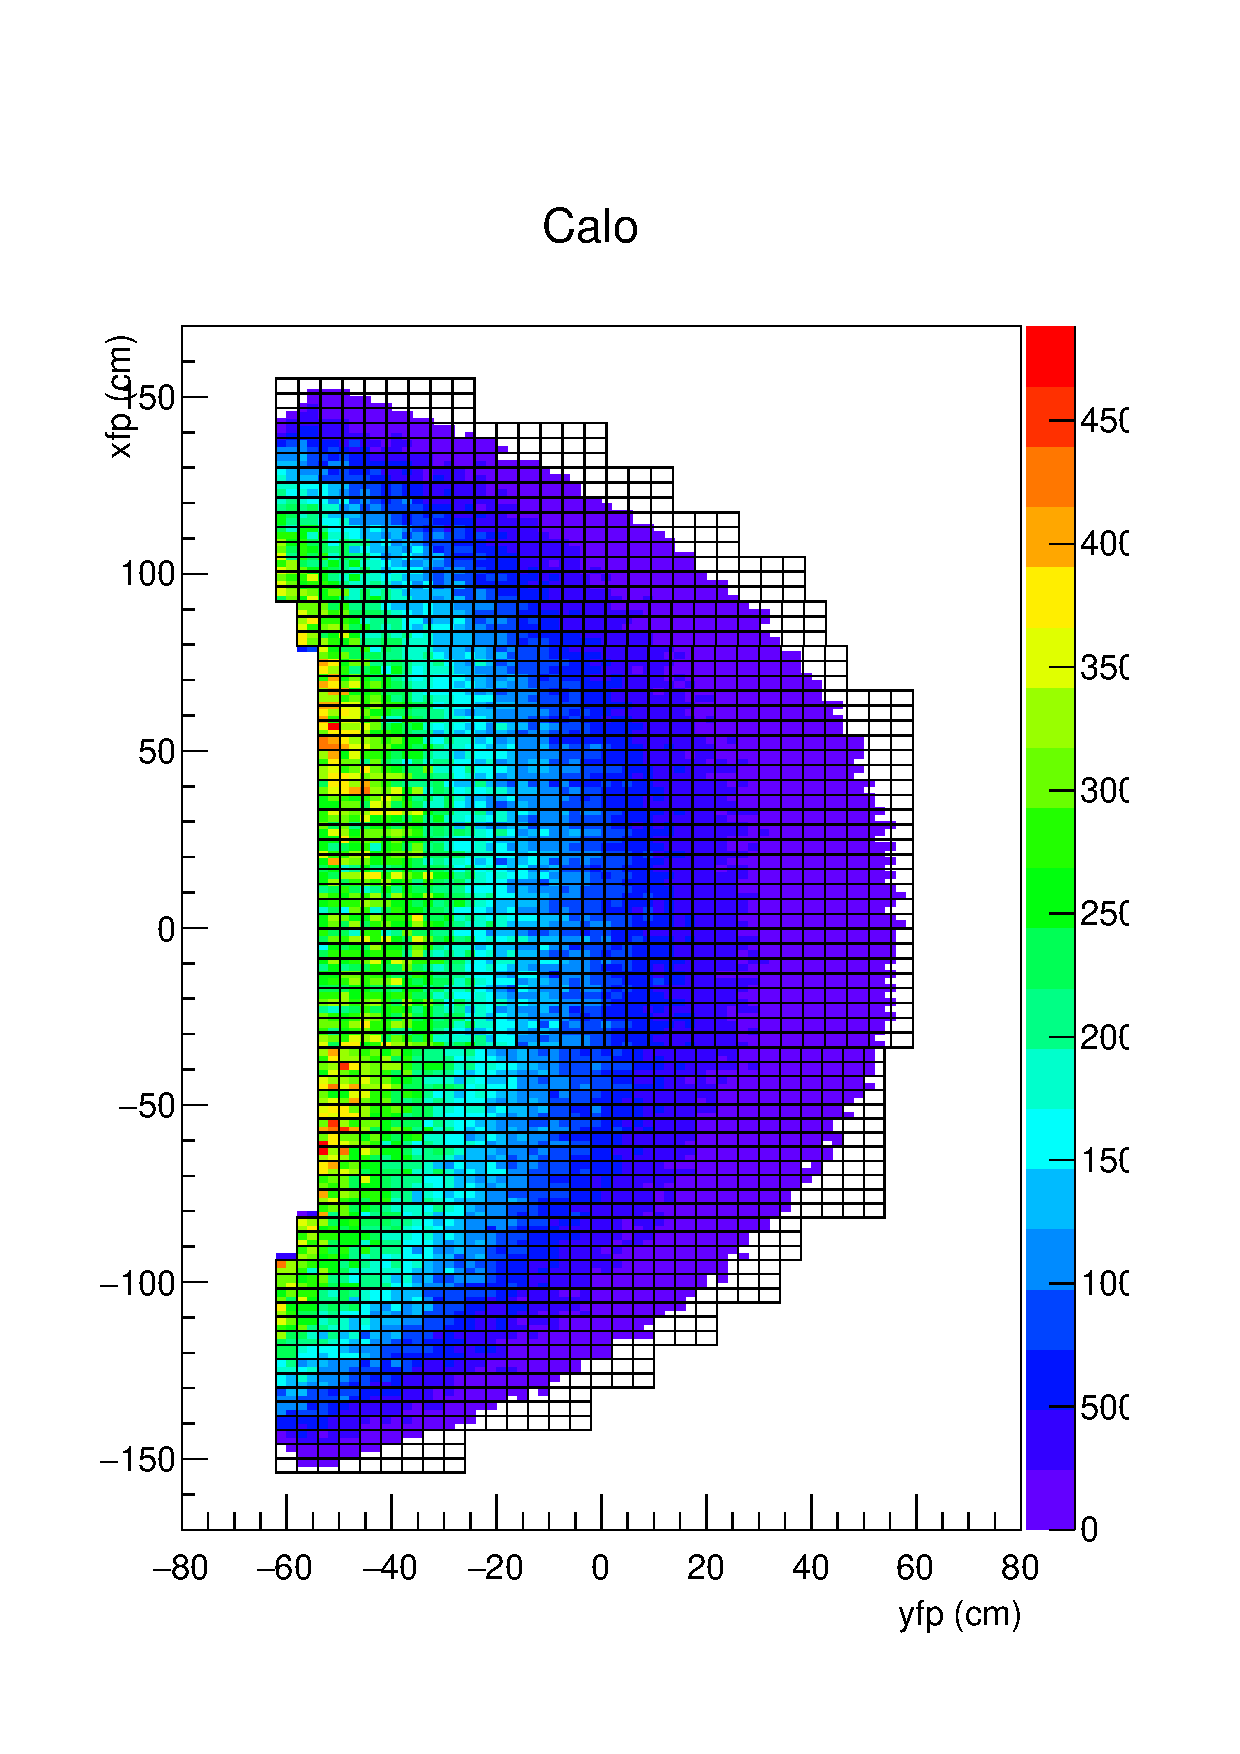
\includegraphics[width=0.3\textwidth]{cfpbox.pdf}
 	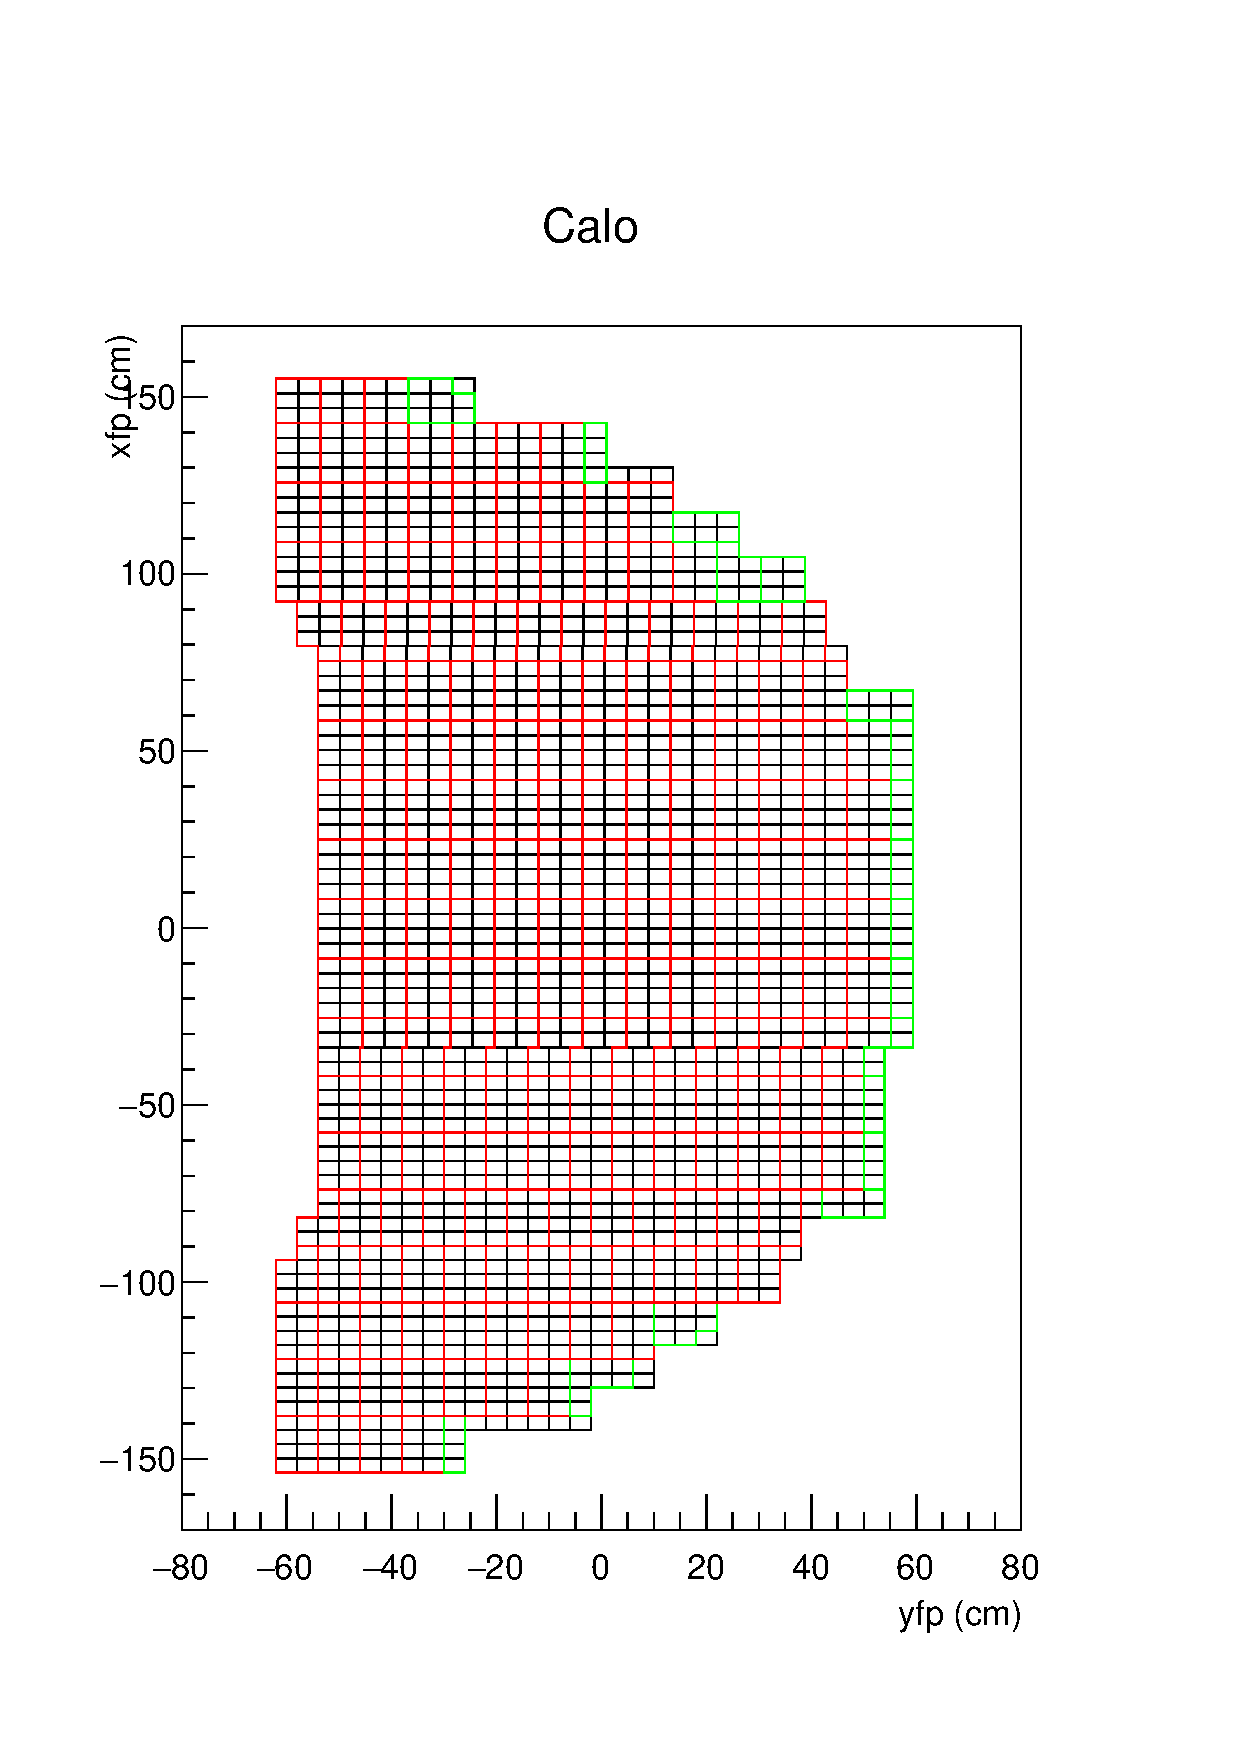
\includegraphics[width=0.3\textwidth]{cfpc.pdf}
 	 	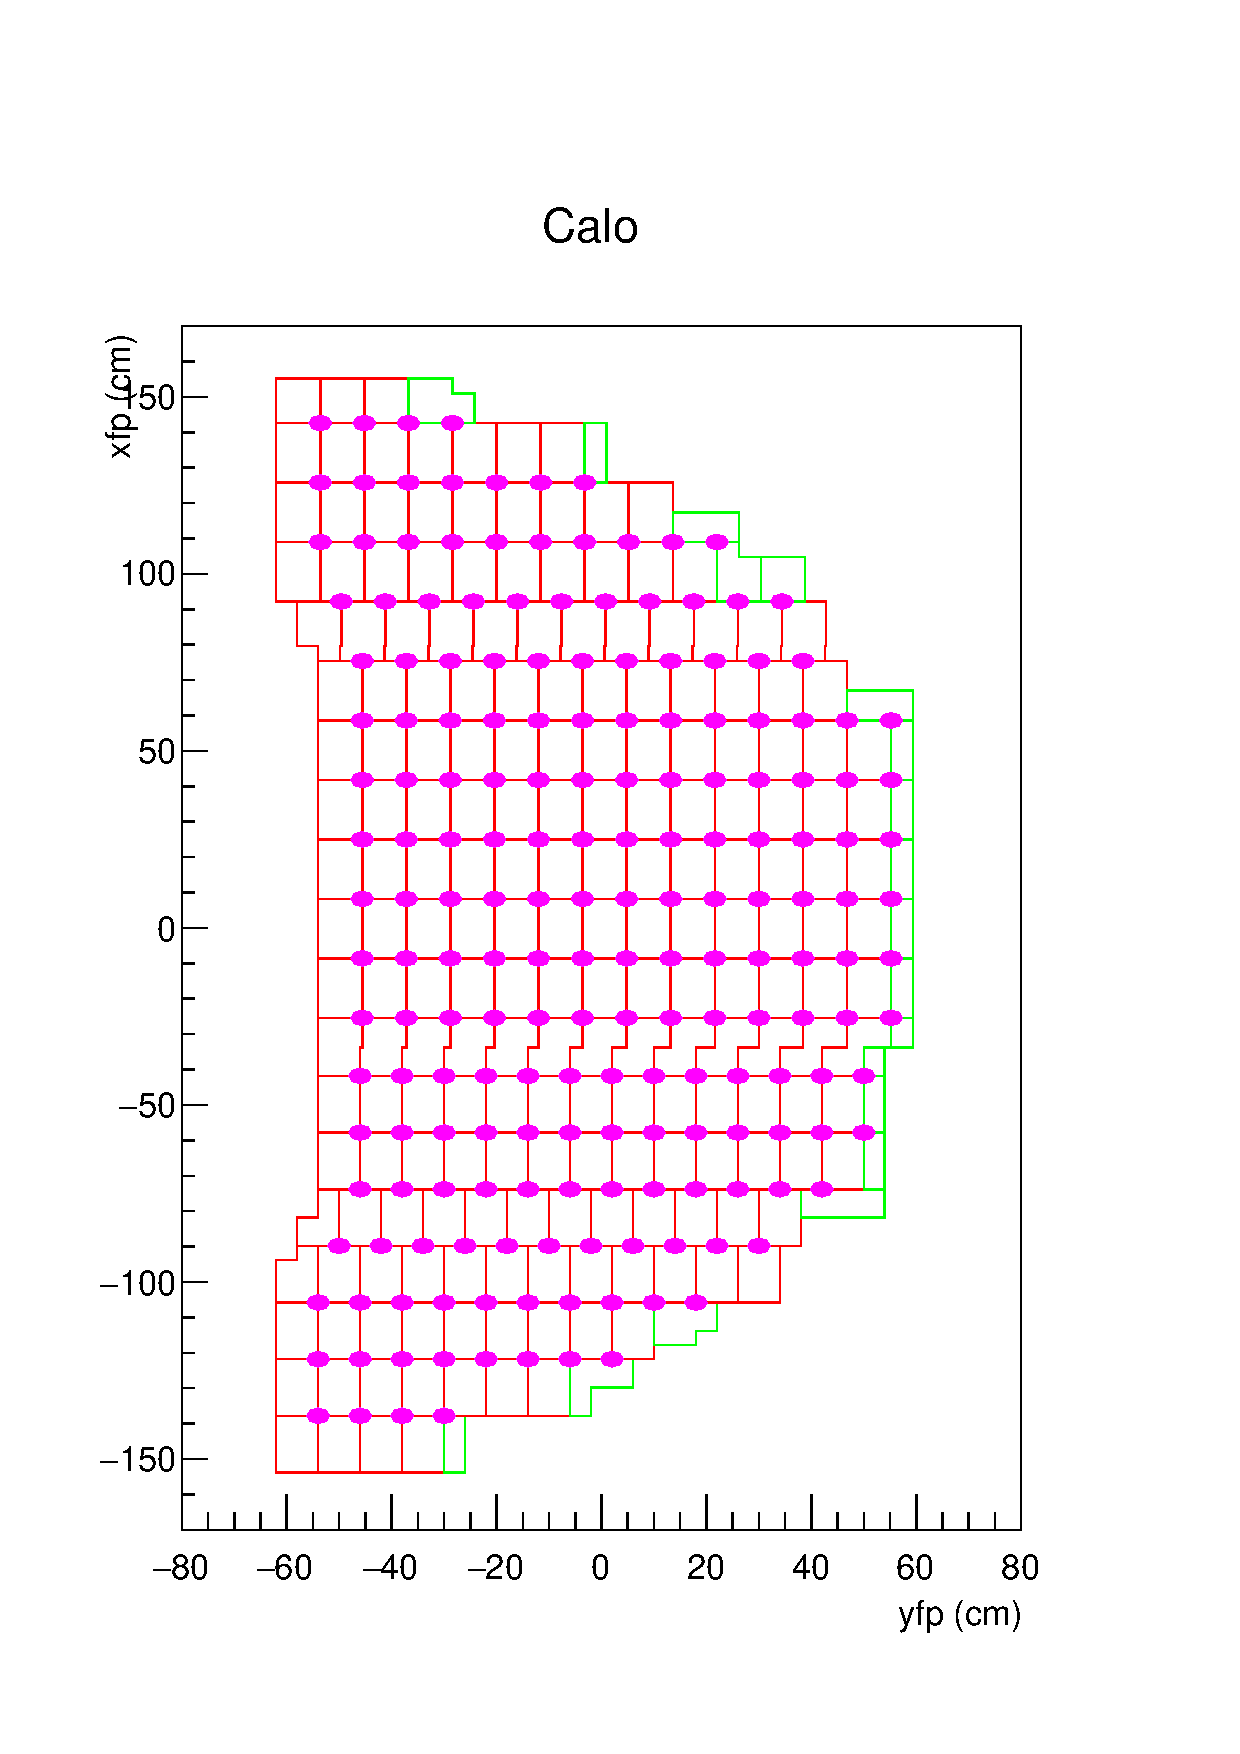
\includegraphics[width=0.3\textwidth]{cgr32.pdf}
 	 	\caption{The left plot is the distribution of elastic electrons in ECAL with the black rectangles representing
 		groups of 2x4 lead glass blocks. The right plot demonstrates
 		the scheme for make overlapping groups of 32 lead glass blocks to be used in the ECAL trigger with
 		details explained in text.  }\label{fig:ECALTrig}
 \end{figure}
 
\end{document}


